%!TEX TS-program = xelatex
%!TEX encoding = UTF-8 Unicode

\documentclass[11pt,tikz,border=1]{standalone}
\usepackage{graphicx}
\usepackage[default,mdseries=Light,bfseries=Medium,path=fonts]{cjkfonts}
\usetikzlibrary{calc,positioning,arrows.meta,shapes.geometric,shapes.misc }
\usepackage{amsmath}
\usepackage{amsfonts}
\usepackage{amssymb}

\begin{document}
  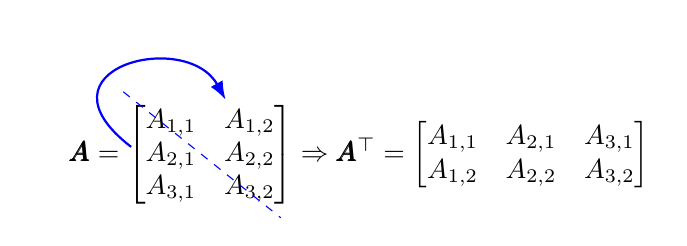
\begin{tikzpicture}
  
    \node(eq) {
      $\pmb{A} = \begin{bmatrix}
        A_{1,1} & A_{1,2} \\
        A_{2,1} & A_{2,2} \\
        A_{3,1} & A_{3,2} \\
      \end{bmatrix} \Rightarrow
      \pmb{A}^{\top} = \begin{bmatrix}
        A_{1,1} & A_{2,1} & A_{3,1} \\
        A_{1,2} & A_{2,2} & A_{3,2} \\
      \end{bmatrix}
      $
    };
    
    \draw[blue,dashed] (-3,0.8) -- (-1,-0.8);
    \draw[blue,thick,-{Latex[]}] (-2.9,0.1) .. controls (-4.2, 1.1) and (-2.2, 1.6) .. (-1.7,0.7);
  
  \end{tikzpicture}
\end{document}
